\documentclass[preprint,pdf]{iucr}
\journalcode{D}
\usepackage{graphicx}
\usepackage{cite}

\begin{document}

\title{Decision Making in xia2}

\author[a]{G.}{Winter}
\author[a]{C.M.C.}{Lobley}
\author[b]{S.M.}{Prince}
\aff[a]{Diamond Light Source, Harwell Science and Innovation Campus,
Oxfordshire, \country{UK}}
\aff[b]{Faculty of Life Sciences, Manchester Interdisciplinary  Biocentre, 
Manchester, \country{UK}}

\keyword{automation}
\keyword{data reduction}
\keyword{expert system}

\maketitle
\clearpage

\begin{synopsis}
The basis for decision making in the program \emph{xia2} is described,
also giving guidelines which can be applied in interactive data processing.
\end{synopsis}

\begin{abstract}

The usage of the data reduction expert system \emph{xia2} was
presented in an earlier article \cite{Winter:ea5113}. Here the decision making
protocols employed in the system are presented, with a discussion
of how these were determined, and how they may be applied in interactive
processing. 

\end{abstract}

\section{Introduction}

Decisions made during interactive data reduction are typically based
on experience, advice from program authors and other users. In many
cases this will work, reinforcing the strategy, and it is typically
only when these fail that more detail about those choices is
sought. Equally, suggestions from the program authors rarely include a
systematic appraisal of the possibilities and explanations as to
which options will work best and why. 
In the development of \emph{xia2} this absence was found
to be a limitation giving rise to a systematic investigation of the best
options for a number of programs, 
based on an analysis of data from the Joint Centre
for Structural Genomics\footnote{http://www.jcsg.org} (JCSG.) The
outcomes of this investigation will be described here, along with the
expert system \emph{framework} in which the decision making was
embedded to develop the final data reduction tool, \emph{xia2}.

\subsection{Workflow}

Taken from the top level, the workflow of data reduction for
macromolecular crystallography (MX) can be considered as three phases:
(i) characterisation and (ii) integration of data from individual sweeps,
followed by (iii) scaling and merging of all sweeps taken from a given
crystal. Decisions made at earlier stages has implications for
subsequent stages, and information from the later stages may
contradict those earlier decisions. Any system to automate data
reduction must therefore be sufficiently flexible to manage this
situation gracefully, considering all decisions made as hypotheses
that are subsequently tested. The system must also embody the workflow being
performed to give the structure into which to embed the decision
making expertise.

\subsection{Blueprint}

For any given choice there may be a set of optimum parameters for a
specific example data set. There may however also be a set of
parameters which can be 
shown to generally work well with limited knowledge of the problem in
hand, for example a general ``class'' of data sets.
These \emph{guidelines} may be determined from a systematic
analysis of a number of data sets, which should ideally be free of
artefacts. This criterion highlighted the value of data from 
structural genomics programs, where the published data are well
characterised (i.e. the structure has been solved) and have been
collected in a consistent manner. This has the benefit that the
decision making may focus on the crystallograhic choices, without
needing to work around problems caused by poor sample quality or
inappropriate choices in data collection. 

Finally, it is important to recognise that software for MX is
constantly evolving, and that new packages will become available which
ideally should be incorporated into the system. As such, some emphasis
on abstraction of steps in the workflow is also helpful, to allow
existing components within the system to be replaced. Currently \emph{xia2} 
includes support for two main integration packages, Mosflm
\cite{leslie1992rcm} and XDS \cite{Kabsch:dz5179}
which are accessed as the 2D and 3D
pipelines respectively, reflecting the approach taken to profile
fitting. These are used in combination with Scala \cite{Evans:ba5084}, XSCALE
and more recently Aimless (Evans and Murshudov, this volume) as well
as other
tools from the CCP4 suite to deliver the final result. In
addition, Labelit \cite{Sauter:dd5008} and CCTBX
\cite{Grosse-Kunstleve:ks0118} are also 
extensively used in the analysis.

\section{Decision Making for Data Reduction: Characterisation}

As discussed above, the crystallographic workflow is considered within
\emph{xia2} in three phases - characterisation, integration and
scaling. Within each of these there will be decisions which need to be
made as well as decisions as to how to handle passing information
around the system, in particular from later stages to earlier. 

Here, the decisions \emph{within} each phase will be considered for
each of the software packages supported, including special cases and
advice the user about appropriate \emph{xia2} options to use where
appropriate. The objective of the characterisation stage is to determine:

\begin{itemize}
\item{A list of possible Bravais lattice options and appropriate cell
    constants for each.}
\item{Refined / updated values for the beam centre and distance.}
\item{A lattice / cell proposal, based on an analysis of the possible
    options.}
\end{itemize}

\noindent
for a given sweep of images. In addition, any crystal orientation
matrices calculated
should also be available. For a given program, the choices to make
are: the selection of images to use for indexing, the thresholds to
use for indexing, selection of the ``best'' solution and analysis to
ensure that the selected solution appears to be satisfactory. 

\subsection{Labelit and Mosflm}

Labelit and Mosflm share the same underlying one-dimensional FFT
indexing algorithm \cite{Steller:mf0013} though the
implementation in Labelit allows for an additional search to refine
the direct beam centre over a wider range. As such, the behaviour of
the programs in indexing is similar, requiring only one analysis for
the selection of images - though the analysis of solutions will depend
on the program being used as they are scored differently.
The authors of both Labelit and Mosflm recommend the use of two images
for indexing, spaced by $\sim 90^{\circ}$ in rotation\footnote{Subsequently
referred to as $\phi$ for brevity} giving a wide coverage of
reciprocal space over which to determine the basis vectors. 

To optimise any process a scoring scheme is needed. Here the objective
is to determine the selection of images which generally give the most
accurate indexing solution. As the R.M.S. deviation between observed
and predicted spot centres is a target of refinement and the ideal absolute
values of the unit cell constants are poorly defined (at least at this
stage) these represent poor metrics. The metric penalty however,
defined as the deviation from the constraints for each Bravais lattice
\cite{Grosse-Kunstleve:sh5006} is appropriate as this is a test for
internal consistency 
and is also relevent for automatic strategy systems such as EDNA
\cite{Incardona:wa5014}. With this in mind, a secondary constraint is raised:
there is a benefit in using few rather than many images.

\begin{figure}
\caption{Mean normalised metric penalty as a function of number of
  images used for characterisation with Labelit, where smaller values
  indicate more accurate solutions.
\label{figure:no_images}}
\centering
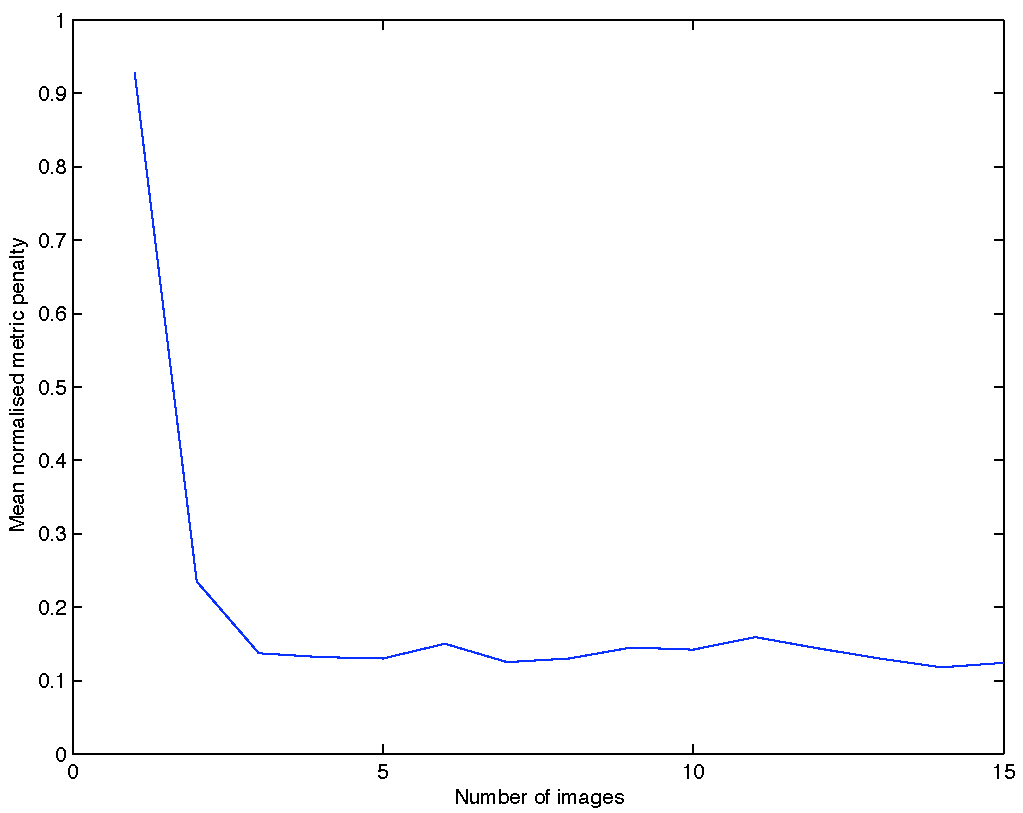
\includegraphics[scale=0.5]{figures/no_images.pdf}
\end{figure}

Data were taken from 86 sweeps from the JCSG archive, where  the
following four
criteria were met: the lattice was not pseudosymmetric, nor triclinic,
autoindexing with a single image gave the ``correct'' result and at
least $90^{\circ}$ of data were available. First, the number of images
to use for indexing was considered. Figure~\ref{figure:no_images}
shows the mean 
normalized metric penalty\footnote{All of the metric penalties for a
  given sweep were scaled over the range $0 - 1$, then this normalized
  value averaged across all sweeps for a given number of images.} for
one to 15 images spread across the range $0 - 90^{\circ}$, where
smaller values indicate a more accurate solution. Clearly the use of
two images gives a substantially more accurate result than the use of
a single frame, confirming the advice from the Mosflm and
Labelit authors. However a further improvement may be observed from
using three images, after which no further improvement is clear. 

\begin{figure}
\caption{Normalised metric penalty for indexing from three images, up
  to a maximum spacing of $45^{\circ}$.
\label{figure:phi_spacing_45a}}
\centering
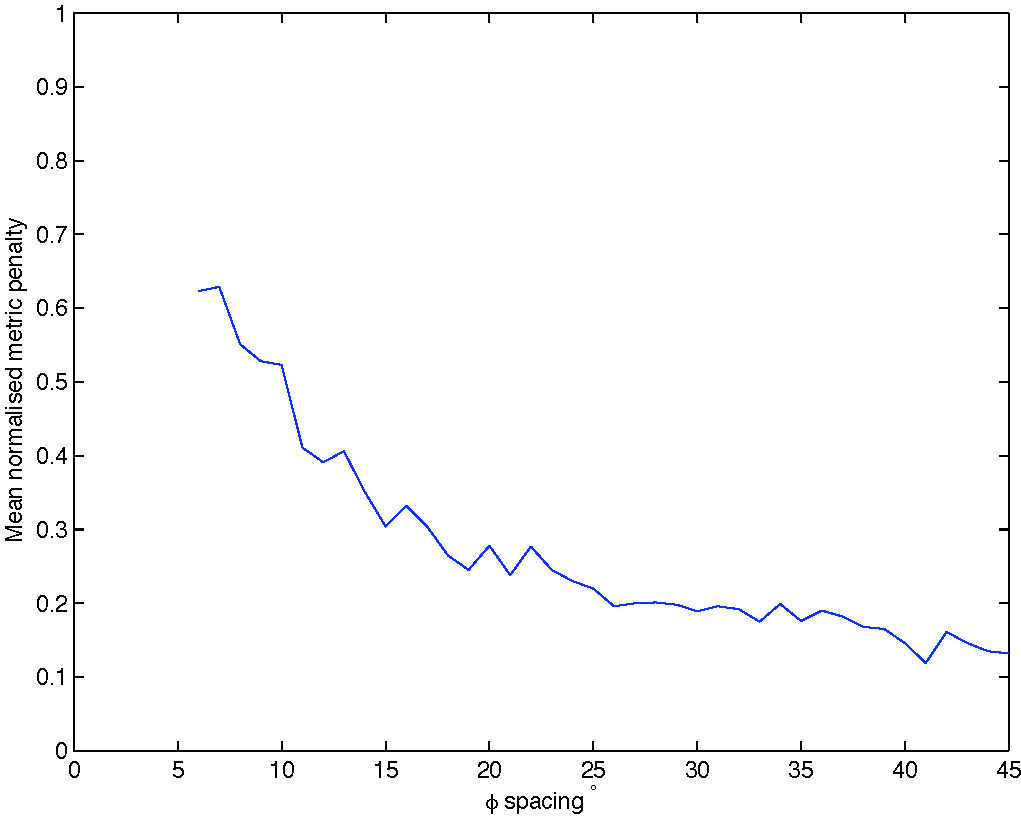
\includegraphics[scale=0.5]{figures/phi_spacing_45a.pdf}
\end{figure}

Following a similar procedure it was found
(Figure~\ref{figure:phi_spacing_45a}) that a 
spacing of $\sim 45^{\circ}$ generally gave the most accurate
solution. Extending this analysis to sweeps of up to $180^{\circ}$
confirmed this result (not shown.) 

This result may be considered as follows: the one-dimensional FFT
indexing procedure employed in Mosflm and Labelit computes the
Fourier transform of the projection of the observed peaks gathered
from all images in $\sim
7000$ reciprocal space directions. Those directions which show the
strongest signal are then considered as possible basis vectors. Using
three images spaced by $\sim 45^{\circ}$ ensures that every reciprocal
space direction is likely to be well sampled. This will make it more likely
that a fundamental basis vector, rather than some linear combination
of basis vectors, will be found giving a more accurate result.

When using Labelit, the proposed solution is chosen to be the highest symmetry
Bravais lattice / cell combination highlighted in the output. The
Bravais lattice / cell combinations for all other lattices are also
recorded, where the cell is chosen to be the one with the lowest
metric penalty where multiple options exist. In usual operation Mosflm
makes a selection from the possible solutions which satisfies similar
constraints, which is taken by \emph{xia2}. Once again, all possible
options are saved. It is important to note that this selection of the
highest symmetry plausible solution is reasonable as it will be
substantially challenged in subsequent analysis steps.

\subsection{XDS}

Unlike Mosflm and Labelit, the indexing in XDS uses $\phi$
centroids as well as positions on the image of reflections, and
therefore operates most reliably when given one or more \emph{wedges} of
images. Indeed, it is perfectly possible to index with peaks taken
from every image in the sweep, a process which may be desirable in some
circumstances. The indexing algorithm is however less robust to
errors in the direct beam position than the procedure in
Labelit. The usual procedure in \emph{xia2} is therefore to first
index with Labelit and repeat this indexing with XDS
using the refined beam centre and selected cell and symmetry. However
this behaviour is under the user's control \emph{via} command-line
options which are listed in the \emph{xia2} manual.

Where Mosflm and Labelit make explicit assumptions about the experimental
geometry, XDS allows a general rotation axis and beam vector and will
typically refine these during the indexing step. Therefore, if the
intention is to use XDS for integration it is necessary to
repeat the indexing of the data if Labelit or Mosflm were used for the
initial characterisation. Determination of the optimum
selection of images for indexing with XDS is therefore necessary.

\begin{figure}
\caption{Mean normalised metric penalty for the correct autoindexing 
solution from XDS, as a function of the number of $5^{\circ}$ wedges used.
The 0 point corresponds to the use of all images. From these results it is
clear that the use of three wedges, rather than the full data set, works
well.
\label{figure:xds_n_images}}
\centering
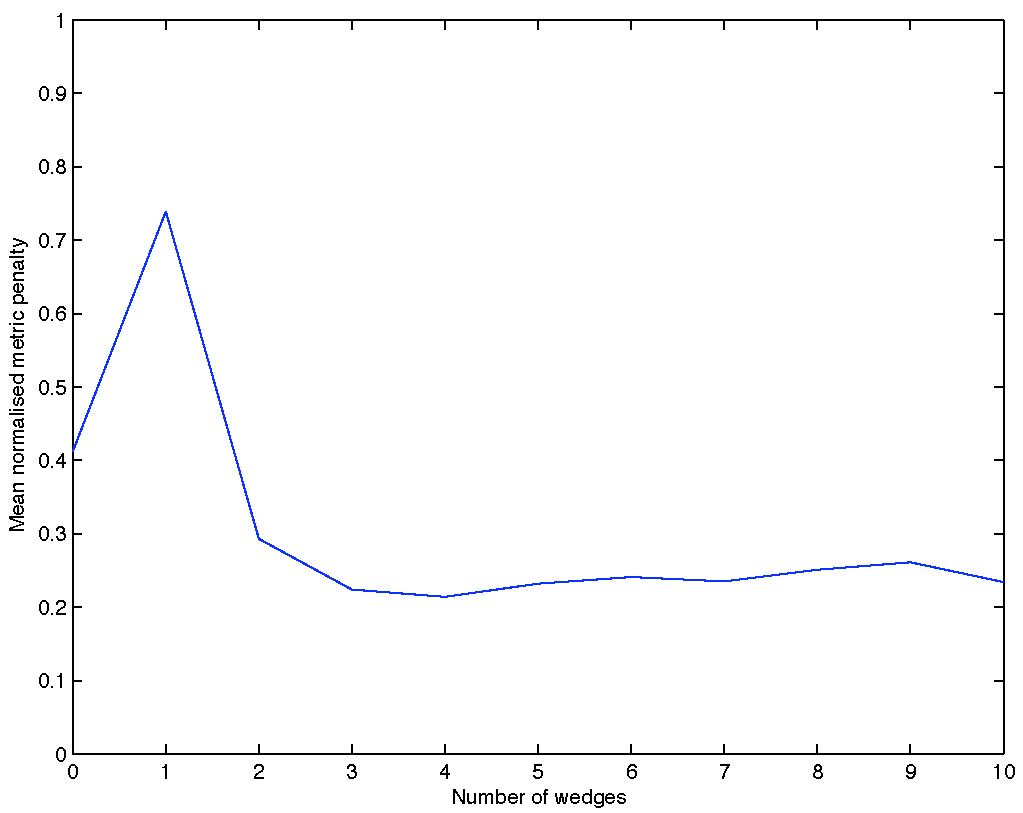
\includegraphics[scale=0.5]{figures/xds_n_wedges.pdf}
\end{figure}

By anology with Labelit, data were indexed with a triclinic basis
from all images and from one to ten $5^{\circ}$ wedges, with the
resulting triclinic cell used with \verb|iotbx.lattice_symmetry| to
compute the metric penalty for the correct lattice. As may be seen
from Figure~\ref{figure:xds_n_images},
use of a single $5^{\circ}$ wedge gave the poorest
results followed by the use of all images. The use of two and three
wedges gave further improvement, with no improvement observed
subsequently. Following from this, various wedge sizes were tested and
no substantial trends, beyond using at least two frames, were found
though a slight benefit was observed for using $\sim 5^{\circ}$ wedges
(not shown.) Finally the ideal spacing was found to be $\sim
45^{\circ}$ though little improvement was found beyond $\sim
20^{\circ}$ (also not shown.)  

In the case that XDS is used for the initial indexing, it is necessary
to select a proposed solution from the 44 lattice characters output by
XDS. In the analysis no solutions with a penalty higher than 40 were
found to be correct, so with no guidance the system will select the
highest symmetry solution with a penalty lower than this threshold. If
however the symmetry has been given by the user this limit is raised
to 200. As with Labelit, in cases of multiple cell possibilities for a
given lattice the one with the lowest penalty is chosen.

% got as far as here

\section{Decision Making for Data Reduction: Integration}

The objective of the integration step is to:

\begin{itemize}
\item{Accurately measure the intensities of the reflections.}
\item{Validate the results of characterisation, i.e. test whether the
    lattice assigned in the characerisation step is appropriate.}
\item{Provide a refined model for the experimental geometry and
    crystal lattice.}
\end{itemize}

\noindent
While these objectives have been listed in order of decreasing
importance to the structure solution process, the second is perhaps
most significant the development of an expert system. When processing
interactively for example using iMosflm it is
straightforward to see if the indexing solution is appropriate from a
comparison of the observed and predicted reflection positions. When
the analysis is performed with nothing in the way of visual feedback,
as is the case inside \emph{xia2}, an equivalent assessment is
needed. This assessment depends on the program used, and will be
discussed shortly.

\subsection{Mosflm}

A typical interactive integration session with Mosflm will start with
indexing followed by the refinement of the cell, once the lattice has
been chosen. At this stage the integration may be performed either
through the GUI or from a script. However, by working through this
process a great deal of information about the data has been learned by
the program, for example spot profle parameters from the spot search
prior to indexing. In automating this analysis, particularly when
alternative programs may be used for some of the steps, some effort
must be made to reproduce the program state. This, coupled with the
cell refinement step, may be characterised as preparation for
integration. The decision making will therefore be separated into
preparation for integration and integration proper.

The preparation for integration is primarily to set up Moslfm into
a suitable state for performing integration. This will require the
selection of images for the cell refinement and
the configuration of the program state. To determine rules for the
selection of images a similar process was followed to the selection of
images for indexing with XDS, allowing for an additional constraint of
the use of 30 frames or fewer in cell refinement, with a similar
conclusion. In essence, the cell refinement was performed in P1 for the
sweeps used earlier, and the resulting cell constants scored
\emph{via} metric penalty, resulting in the use of three small wedges
of data spaced by ideally $45^{\circ}$. To robustly prepare the program state
for cell refinement however it is necessary to first gather the
reflection profile parameters that would usually be obtained during
indexing. To achieve this an incidental indexing step is
performed, where the spot parameters and an estimate of the resolution
limit are retained from the program output
but the other results ignored. It was found that
applying this rather conservative
resolution limit during the cell refinement gave rise to
much more reliable results.

To approximate the visual assessment described above, the cell
refinement is performed with the proposed lattice from
characterisation and with a triclinic 
basis, with the orientation matrix from
characterisation transformed appropriately. When the R.M.S. deviations
between the observed and predicted spot positions are compared in a
pairwise manner (i.e. as a function of frame number and refinement
cycle) between the proposed and triclinic lattices
a ratio may be calculated. It was found that in
all cases when the lattice had been correctly assigned this ratio was
less than 1.5. However, in cases where the lattice had pseudosymmetry
(i.e. monoclinic with $\beta \sim 90^{\circ}$)
the ratio exceeded this value, and 1.5 is therefore used as a
cutoff. Intuitively this makes sense: if the application of the
lattice constraints makes the aignment of the predictions with the
observed spot positions 50\% worse the lattice constraints are
unlikely to be correct. If this is the case that solution may be
eliminated from consideration and the next lower symmetry lattice
considered, a process which takes place within the characterisation.
Other tests, such as comparing the deviation of the refined triclinic
cell constants to those satisfying the lattice symmetry as a function
of the estimated standard deviation of those constraints was found to
be unreliable. Once the preparation is complete there are a number of
choices to be made for the integration proper:

\begin{itemize}
\item{Whether to fix the cell constants during integration.}
\item{Whether to perform the integration with the lattice constraints
    applied, as recommended by the Mosflm authors, or with a triclinic
    basis.}
\item{Whether to apply a resolution limit during integration,
    as opposed to integrating across the entire active area.}
\end{itemize}

Wheras the previous choices have been assessed in terms of the accuracy
of the resulting cell constants, here the metric will need to relate
to the accuracy of the observations, best observed by scaling the data
and considering the merging statistics. Provided that the extent of
the data are unchanged (i.e. same image range, same resolution limits)
$R_{\rm{merge}}$ will be a reliable indicator of accuracy. To make
this assessment, Pointless \cite{Evans:ba5084} and Scala were
used, the latter with a ``standard'' scaling model\footnote{Smoothed
  scaing on rotation with $5^{\circ}$ intervals, secondary absorption
  correction and smoothed $B$ factor correction with $20^{\circ}$
  intervals.}
(the default in CCP4i.) Protocols were determined for integration to assess each
of the above choices, by comparison with the procedures recommended
by the program authors. In summary, it was found that fixing the cell
constants during integration was helpful however applying a resolution
cutoff made little difference, as did applying the Bravais lattice
constraints. The conclusion was therefore to integrate across the
active area of the detector, fixing the cell constants and applying
the lattice constraints, though in hindsight there are arguments
against the latter and developments are underway to perform all
processing in with a triclinic basis.

\subsection{XDS}

Where Mosflm is typically run through the graphical user interface
iMosflm, XDS is run on the command-line with a plain text input file,
making it ideal for usage 
within an automated system. The advised use of XDS is to perform all
processing with a triclinic basis, then apply the Bravais lattice
constraints at the final step (i.e. in the postrefinement and scaling.) However it
is possible, but by no means mandatory, to ``recycle'' parameters from
the later stages of processing and rerun the integration. The aim here
is to determine the choices which will generally give rise to the best
quality results, ideally at minimal computational cost. As with the
analysis of integration strategies using Mosflm, $R_{\rm{merge}}$ will
be used as a metric for the quality of the data reduction. The four
choices are:

\begin{itemize}
\item{Whether to enforce the Bravais lattice constraints.}
\item{Whether to recycle the reflection profile parameters.}
\item{Whether to recycle the orientation matrix and experimental
    geometry model.}
\item{Whether to recycle all results of postrefinement including local
    detector distortions.}
\end{itemize}

\noindent
These may be compared with the straightforward protocol described above. Using
the same data as were used for Mosflm, it was
clear that any of these changes to the strategy were ``polishing'' the
data, with an average change in $R_{\rm{merge}}$ of around 2\% of the
value. The only marked improvement was found from recycling the
reflection profile parameters, however it will then be necessary
to reintegrate the full data set.

In processing the data with Mosflm the selection of Bravais lattice
was tested \emph{via} postrefinement. In XDS, global refinement is
performed after integration allowing the lattice to be tested in a
similar manner, once again with a 50\% threshold. Currently in
\emph{xia2} the integration is performed with the Bravais constraints
applied, for historical reasons, though performing the integration
with a triclinic basis is planned. The same global refinement may then
be performed.

\section{Decision Making for Data Reduction: Scaling}

While characterisation and integration operate on sweeps in isolation,
scaling must consider all of the data at once. As such, it is at this
point that all of the processed data are brought together and tested
for consistency, both within individual sweeps (i.e. that the symmetry
in intensity data is consistent with the Bravais lattice) and between
sweeps (i.e. that the Bravais lattices are consistent and that the
data are indexed in a uniform manner.) This requires careful
management of derived information as well as the possibiity for feedback to
earlier processing steps. To assist with this the scaling step is
split into three phases - the preparation, the scaling itself and then
post-processing.

Following the use of Mosflm and XDS, Scala (and now Aimless) and
XSCALE are natural for the main scaling step. However a number of other
programs from CCP4 and elsewhere (including Cad, Truncate and
Pointless) are used to help in this process.

\subsection{Preparation}

\begin{figure}
\caption{Procedure to determine the crystal point group and Bravais
  lattice consistent with the the diffraction data, taking input from
  the indexing and analysis with Pointless.
\label{figure:scaling_1}}
\centering
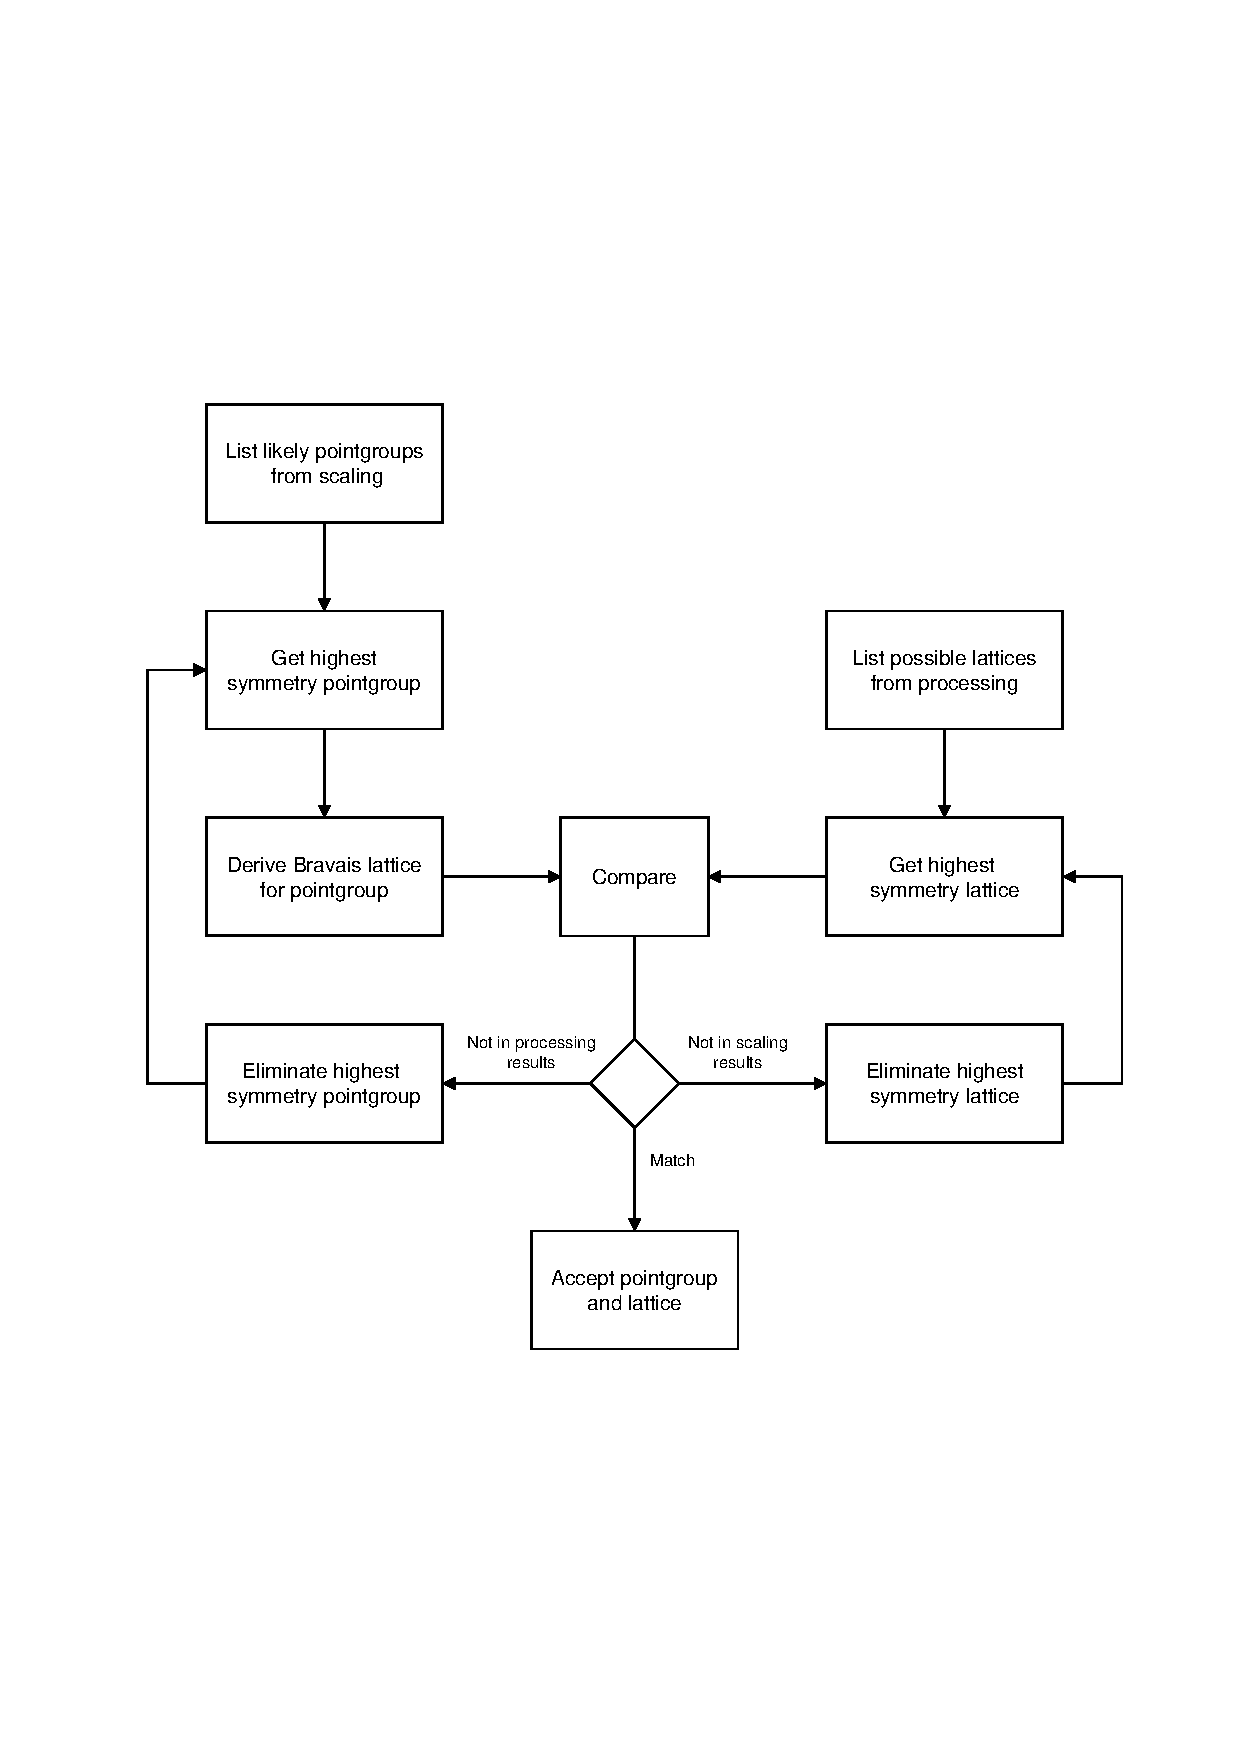
\includegraphics[scale=0.5]{figures/scaling-step-1.pdf}
\end{figure}

In the preparation phase the data from integration are tested for
internal consistency both within and between sweeps. The first test is
to determine whether the Bravais lattice used for processing is
consistent with the apparent pointgroup of the data
(Figure~\ref{figure:scaling_1}.)
This test is performed by comparing the highest allowed Bravais
lattice from processing with the most likely result from Pointless. If
the two are consistent (for example, pointgroup P422 with lattice tP)
the test is passed immediately. If the apparent pointgroup has higher
symmetry than the allowed lattice, as may occur when a
non-crystallographic symmetry axis is closely aligned with the unit cell
axes, that pointgroup is ignored and the next most likely tested. If
however the most likely pointgroup has \emph{lower} symmetry than the
Bravais lattice used for processing the latter is eliminated from
consideration as discussed earlier and the data are reprocessed with
the lattice corresponding to this pointgroup. An example of this would
be a monoclinic lattice with $\beta$ angle indistinguishable
from $90^{\circ}$. 

\begin{figure}
\caption{Procedure for combining pointgroup information from all
  sweeps, following on from \ref{figure:scaling_1}, and assuming that
  the lowest symmetry lattice is correct.
\label{figure:scaling_2}}
\centering
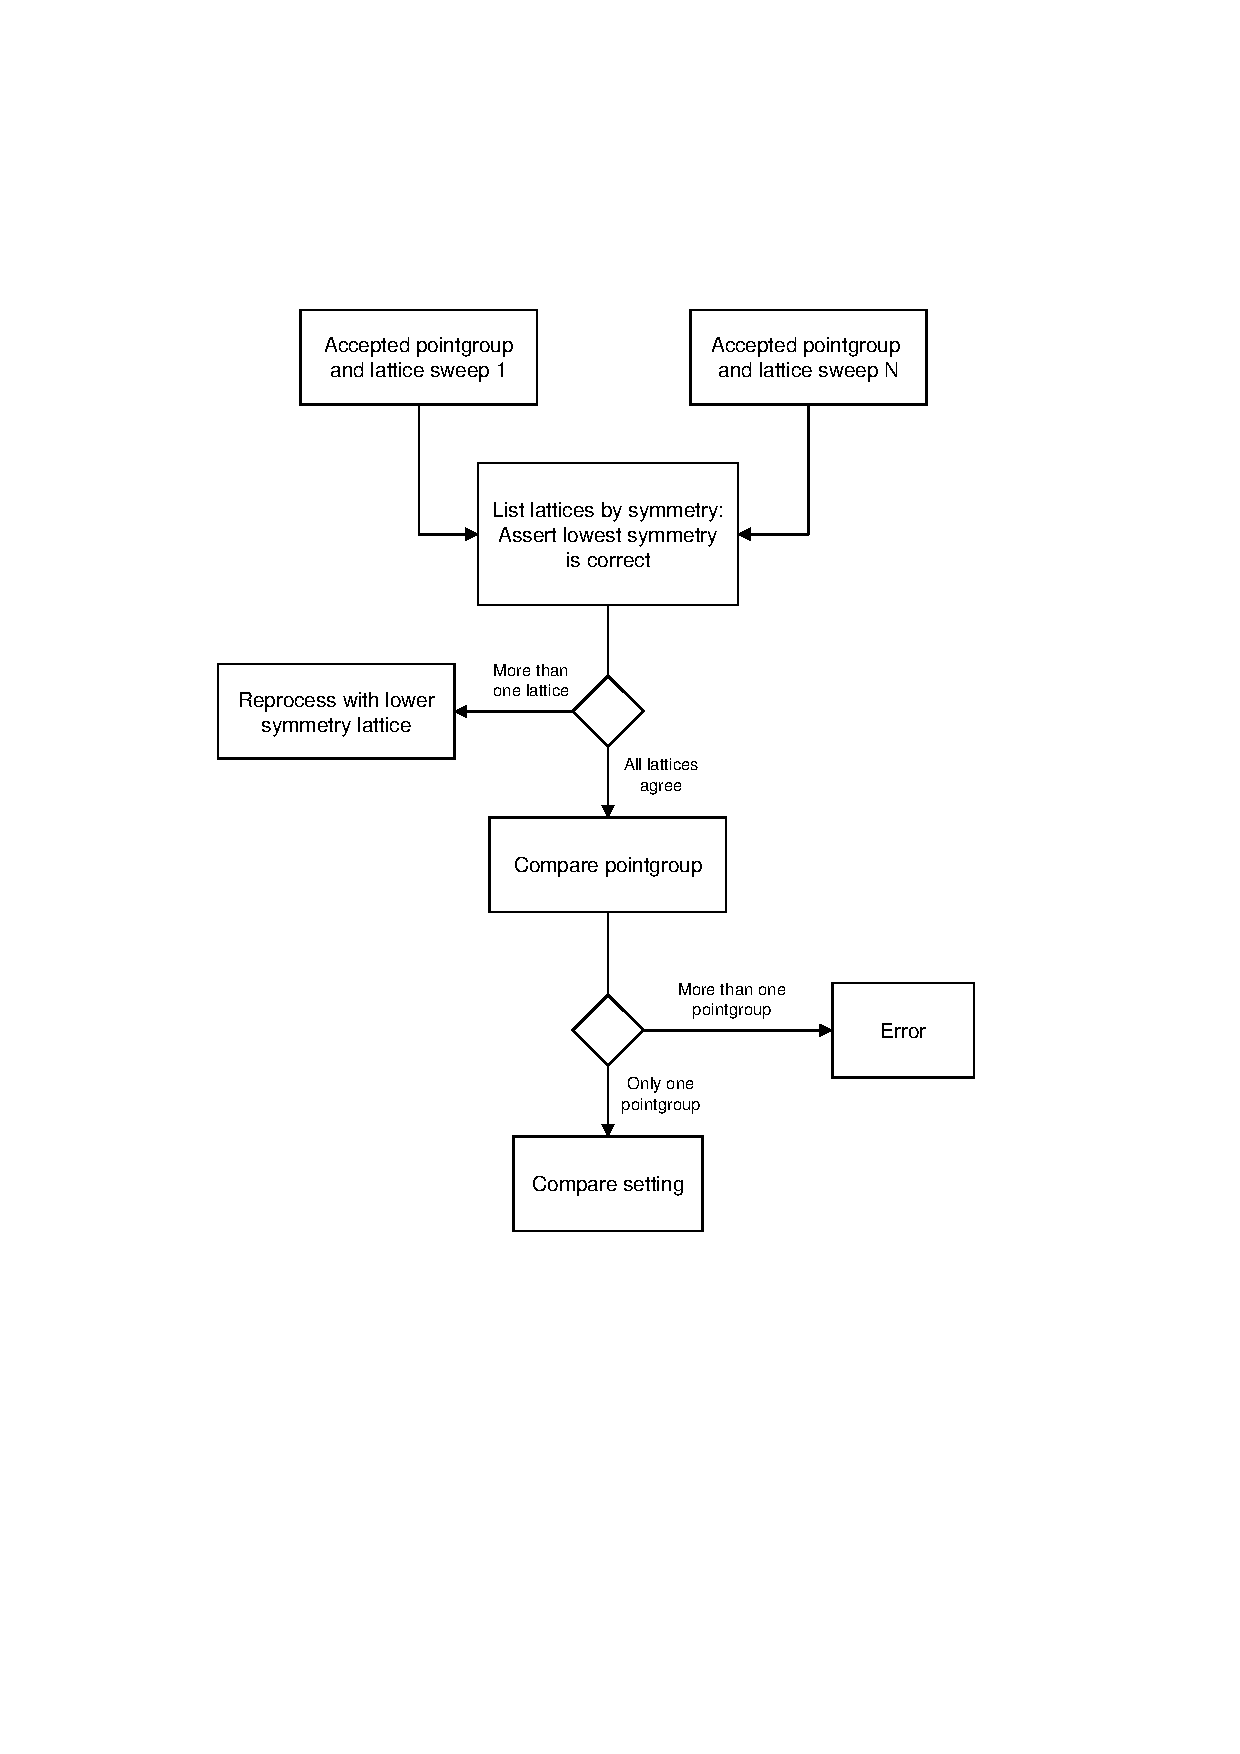
\includegraphics[scale=0.5]{figures/scaling-step-2.pdf}
\end{figure}

Once this test has been passed for all sweeps, the data will have been
processed with a lattice consistent with the pointgroup symmetry of
the data. However, it may be the case (for example from a low and high
resolution pass) that the conclusions for one sweep differ from those
from another. In that case (Figure~\ref{figure:scaling_2}) the lowest
symmetry Bravais lattice\footnote{Defined to be the lattice with
  fewest constraints}
is assumed for all sweeps. If at this stage the pointgroup
conclusions remain inconsistent an error is raised as it is likely
that something has gone wrong - for example an inconsistent data set
has been included in the processing. 

\begin{figure}
\caption{Procedure to establish uniform indexing of all sweeps,
following on from \ref{figure:scaling_2}, which allows for intrinsic
ambiguity in the origin choice where the lattice symmetry is higher
than the pointgroup symmetry.
\label{figure:scaling_3}}
\centering
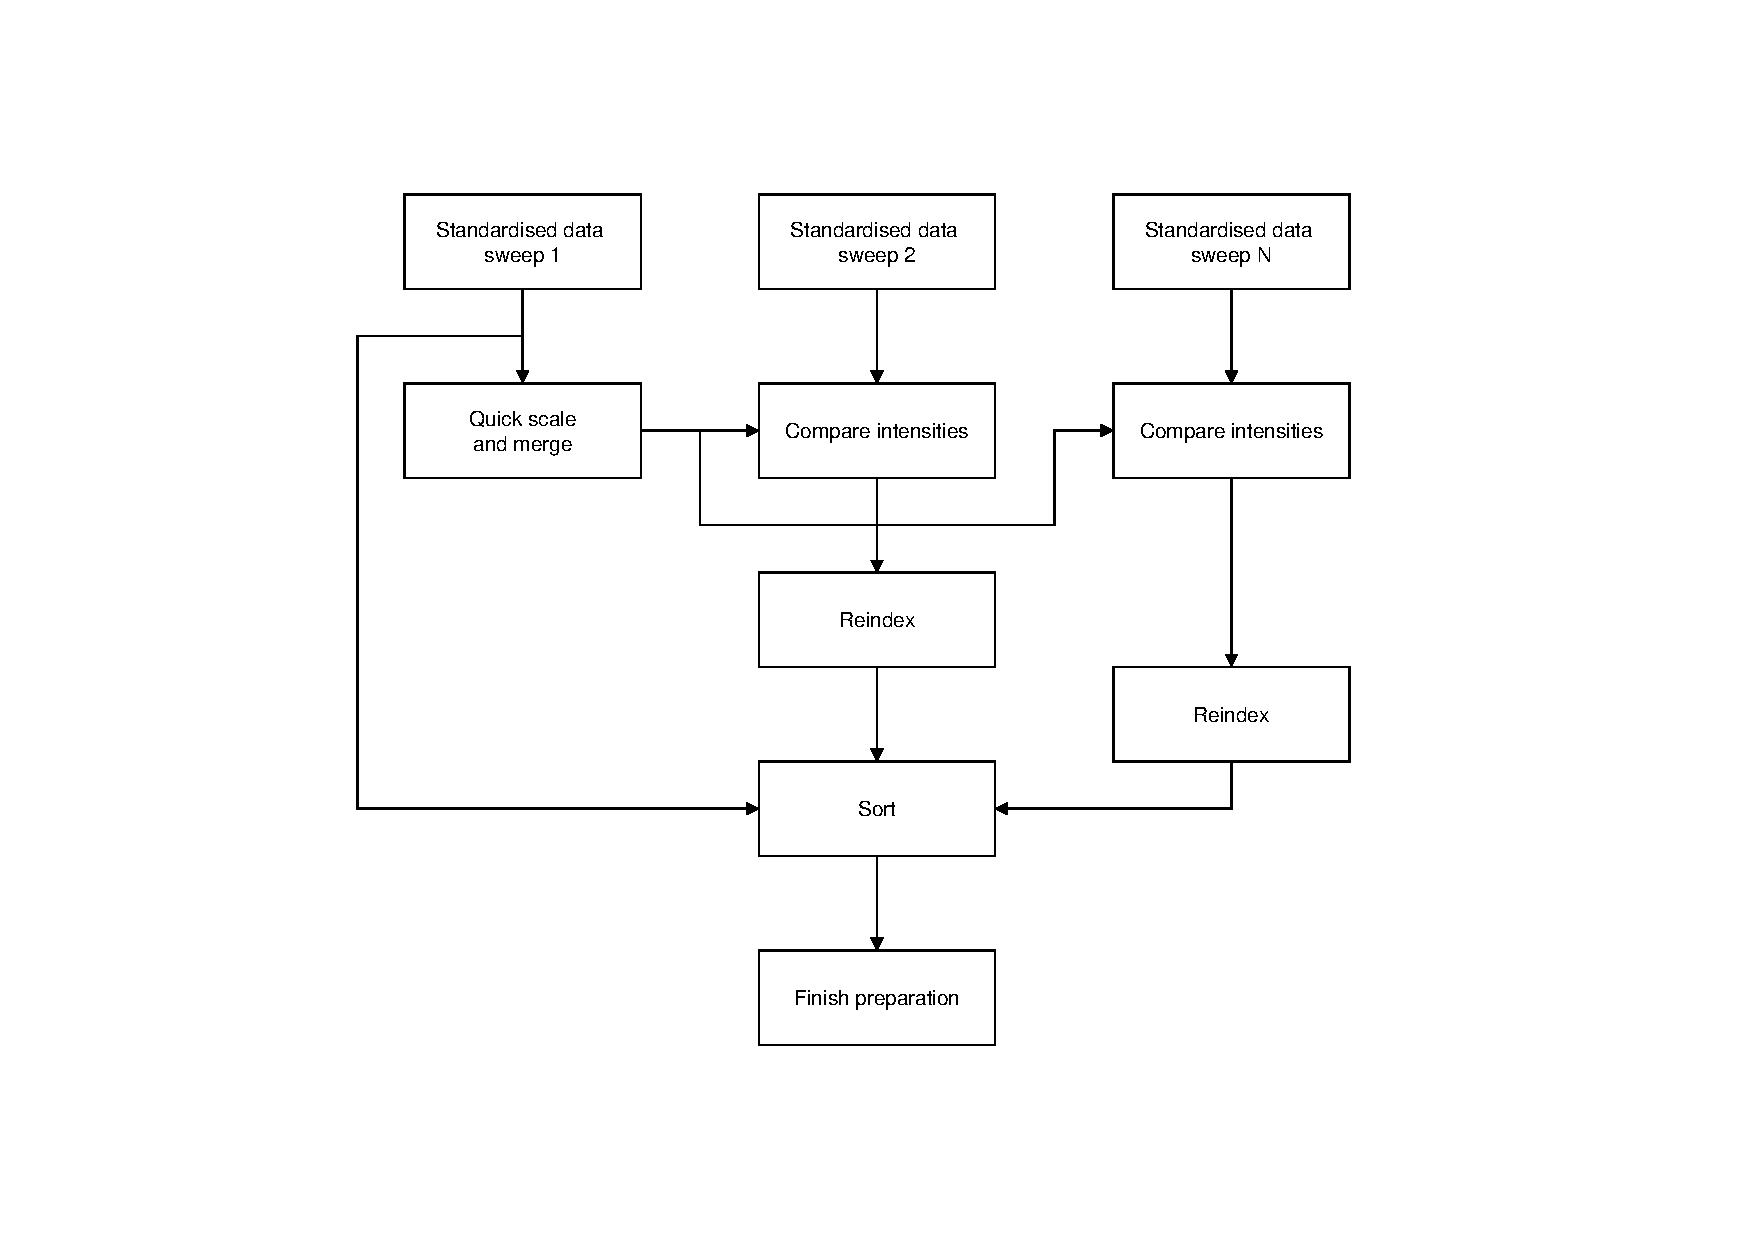
\includegraphics[scale=0.5]{figures/scaling-step-3.pdf}
\end{figure}

Finally, it is necessary to ensure that the data are consistently
indexed to cope with cases where there may be indexing ambiguity,
using Pointless (Figure~\ref{figure:scaling_3}.) At this stage the
most likely
spacegroup is also determined from the systematic absences, primarily
for the benefit of the downstream sructure factor amplitudes, though
often convenient for the program user. When sorting and scaling the
data are put into the sweep order in which they were collected.

\subsection{Scaling with Scala}

Though the scaling protocol recommended in the Scala documentation
(smoothed scales over $5^{\circ}$ spacing in rotation, absorption
correction with 6 orders of spherical harmonics, $B-$factor correction
smoothed over $20^{\circ}$ spacing in rotation) works well in many
cases there are examples when better results may be achieved by,
for example, including the ``tails'' correction or excluding the
decay. As such it is worthwhile to perform a search to decide the most
appropriate model for scaling, which is complicted by the need for a
protocol for decision making. It was found that using Scala
with typical data sets there is essentially no risk of over fitting
the scaling corrections, so the resulting $R_{\rm{merge}}$ was found to
be a reasonable metric as the resolution limits and range of data
considered are unchanged. However, this was found to give an excessive
bias towards corrections for the high resolution data so the low
resolution $R_{\rm{merge}}$ is also taken into account. Finally, in
some cases the combination of scaling corrections may also converge
badly or not at all, which is taken to be an indication of a poor
scaling model. Therefore, 
the resulting protocol uses: scaling with only smoothed scale
factors over $5^{\circ}$ spacing in rotation to give a reference
convergence rate. Then seven other protocols are tested: with and
without decay, absorption and partiality correction, with the model
which gives the best merging residuals while converging in less than
twice the time of the simple run selected. 

In terms of the parameterisation of the scaling, it was found that for
typical data adjusting the rotation range for the scale and
$B$-factors and the number of spherical harmonics used from the
defaults as suggested in the documentation was of little benefit.
Historically, scaling in \emph{xia2} included an iterative process to
determine appropriate correction factors for the error estimates. This
procedure is now performed by Scala and Aimless automatically.

\subsection{Scaling with XSCALE}

Where scaling with Scala applies a parameterised model to the data
in order to minimise the differences between symmetry related
observations, scaling in XSCALE (and the XDS CORRECT step) apply
corrections in terms of arrays of correction values which are indexed
appropriately for decay, absorption and detector modulation. In this
scaling, the principle is to remove correlation of the intensity values
with image number, resolution and detector position, 
respectively. The choice of corrections to apply
is determined by the user.

In the XDS CORRECT step these corrections are applied to each sweep in
isolation. The same corrections are applied in XSCALE to all of the
data simultaneously. It was found that performing the scaling twice
gave no improvement but did effectively double the number of
parameters used, so the choice made in \emph{xia2} is to apply all of
the scaling corrections in XSCALE and apply the minimum in the XDS
CORRECT step. It was found that the application of all scaling factors
(i.e. correcting for decay, detector modulation and absorption)
systematically gives the lowest merging residual so this is the
default choice in \emph{xia2}, though a user option is available to
control this choice. In scaling, all of the sweeps corresponding to
each wavelenth are scaled together but not merged, and
all wavelengths are scaled simultaneously. 

After the initial scaling, resolution limits are calculated
following the procedures set out below, which are then used for subsequent
XSCALE runs. During scaling XSCALE suggests a
list of reflections which do not appear to belong to the data set as a
whole - ``aliens'' - these are subsequently excluded in an iterative manner.

After scaling the unmerged data are reformatted into their original
sweep structure and merged with Scala or Aimless, as this gives an
easily interpreted report on data quality and also a route into
producing MTZ files for the subsequent post processing, discussed below.

\subsection{Resolution Limit Calculation}

Early in the development of \emph{xia2} the resolution limits were
determined from an analysis of the output of Scala, which proved to be
unreliable. Resolution limits are now calculated directly from the
scaled intensity data themselves, using routines developed using
the CCTBX toolbox, allowing the same procedures to be used for data from Scala
and XSCALE, giving more consistent results.

The resolution limit calculations themselves use the merged and
unmerged $\frac{I}{\sigma_I}$ values, the completeness and the
$R_{\rm{merge}}$ as possible criteria for determining a cutoff, with
the first two considered by default with values of 2 and 1
respectively. The cutoff applied to the unmerged data was found to be
helpful when considering data with very high multiplicity - though the
multiplicity provides a boost to the apparent $\frac{I}{\sigma_I}$,
the resulting measurements were found in some cases
to be distributed more like a
normal distrbution than an exponential (i.e. Wilson) distribution as
would be
expected, as judged by the $E^4$ plot from Truncate (not shown.)
This is assumed
to be a result of a poor estimation of the errors for weak
reflections, giving rise to systematic effects in
merging. $CC\frac{1}{2}$ and $CC^*$
have since been proposed as a more robust
choice for resolution limit calculation (Evans \& Murshudov, this
volume and \cite{Karplus25052012})
which will be investigated shortly.

\subsection{Post Processing}

From a certain perspective scaled and merged intensities are the end
product of the data integration and scaling. It is however helpful to
perform a small number of subsequent analysis tasks to prepare the
data for downstream analysis:

\begin{itemize}
\item{Calculation of structure factor amplitudes from intensities.}
\item{Determination of an average unit cell.}
\end{itemize}

\noindent
The former of these uses the ``truncate'' procedure \cite{French:a15572}
where negative intensities are corrected to give small positive
values. However, to best perform this correction it is necessary to
remove systematically absent reflections from the data set, hence the
spacegroup identification performed earlier during the preparation
step. At this stage it is also helpful to get the overall scale for
the amplitudes correct - if the amino acid sequence is provided, the
number of molecules in the asymmetric unit is estimated \cite{KantardjieffRupp}
to give an estimate of the total number of atoms
and hence the appropriate scale factor to apply. In the absence of
this information it is assumed that the unit cell contains 50\%
solvent, with the remaining space filled with ``average'' protein. 

While the determination of the average unit cell is not a fundamental
part of the analysis, it is nevertheless helpful for downstream
calculations. This is computed in \emph{xia2} as an average from the
sweeps, weighted by the number of reflections in each sweep, hence
giving a bias towards higher resolution data sets.

\section{Implementing Automated Data Reduction}

In the previous section the decision making protocols for the data
analysis were considered. These are not however sufficient to allow
automated data analysis, as they need to be embedded in a framework
which encodes the overall strategy for data analysis. In this section
the structure of \emph{xia2} will be described with an emphasis on the
interaction between the analysis and the data.

\subsection{Data Management}

As an expert system can only make decisions based on the information
available, careful management of data is critical. Most data familiar
to macromolecular crystallographers deal with static
information, for example coordinate files and reflection data. 
Within \emph{xia2} however
the knowledge at any stage is a \emph{hypothesis} and hence
subject to change following subsequent analysis. As such it is
important to track the provenance of any derived information, such
that subsequent invalidation of a result (for example, elimination of
an indexing solution) will automatically invalidate any subsequent
conclusions. This \emph{dynamic} information must be treated carefully
to ensure that results are updated when necessary. 

The main information provided to the system is the raw diffraction
data, with suitable metadata (i.e. image headers) to describe the
experiment. In the majority of
cases this information will be sufficient to build
a useful model of the experiment. Within \emph{xia2} the raw data are
structured in terms of sweeps of diffraction data, which belong to
wavelengths (which are merged to a single MTZ data set in the output)
which in turn belong to crystals. The crystals are contained within
projects, but this does not currently take part in the analysis. Crystals
are also the fundamental unit of data for scaling. All of these
data structures (project, crystal, wavelength, sweep) map directly onto
objects within \emph{xia2} and initially contain only static data -
that is, the information derived from image headers or from user
input. However, starting from this input information it is possible to
perform analysis as described earlier, and draw 
conclusions. Although it would be possible to store the results of
this analysis in these data objects, it would be necessary to ensure
that they are kept up-to-date which would generate a substantial
amount of book-keeping. The alternative used inside
\emph{xia2}, is to maintain a link to the
\emph{source} of this information, which is essentially the analysis
task which gave that result. To make this link in a general
way it is necessary to have a standard interface to the analysis
tasks.

\subsection{Expert System Interfaces}

As there are a small number of high level steps in the data analysis
process but a number of possible program options for each, it is
possible to define an abstract interface to describe each step, which
can then be implemented using the existing software 
and the decision making protocols described above. The addition of an
abstract interface also gives the option of centralising standard
decision making steps, for example the management of solutions from
indexing. As an example, both Mosflm and Labelit may be used to index
a diffraction pattern based in a small number of images from a sweep,
so both may present an \emph{Indexer} interface. The detail of how the
indexing is performed and how the results are interpreted will be
program specific and implemented in \emph{MosflmIndexer} and
\emph{LabelitIndexer}, respectively. The application of a standard
interface however allows a standard two-way link to a sweep to be
made, passing in generic information needed for indexing, receiving
generic results from the analysis.

While this approach adds an extra degree of separation between the
data and the analysis programs, it allows for generic aspects of the
analysis to be centralised and the freedom to extend, including
new software as it is developed. 

\begin{figure}
\caption{General flow of expert system interfaces, showing how the
  prepare, do and finish functions are used. Decisions are diamonds,
  processing tasks as rectangles.
\label{figure:fig6}}
\centering
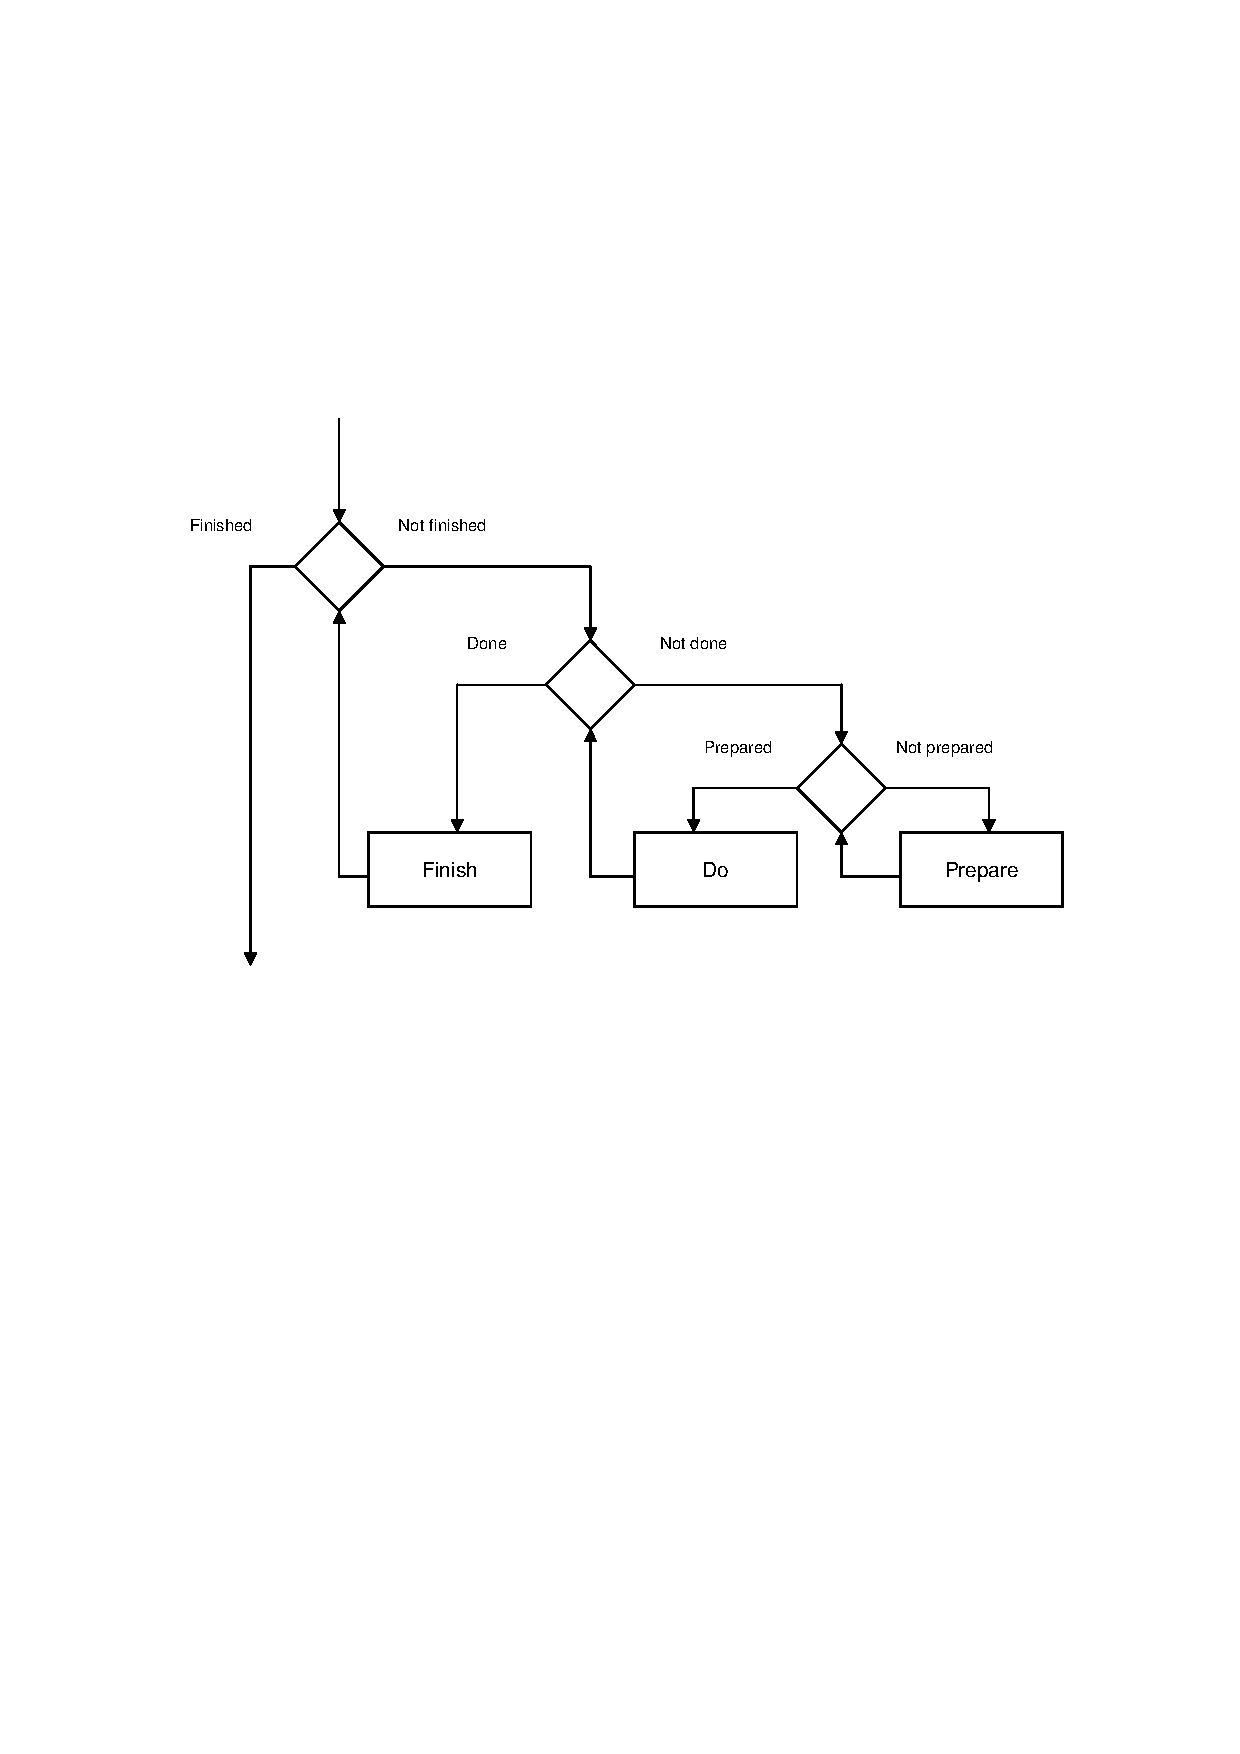
\includegraphics[scale=0.5]{figures/Fig6.pdf}
\end{figure}

Within each interface (\emph{Indexer} and \emph{Integrater}, linked to
sweeps and 
\emph{Scaler} linked to the crystal) there are three standard phases -
prepare, do and 
finish, arranged in a loop (Figure~\ref{figure:fig6}.) 
The status of each phase is
managed internally and each phase will be performed until it is
completed or an error occurs. Once the finish phase is completed any
results which have been derived are assumed valid, however in requests
for information the interface will check that this is the case, and if
not will repeat the necessary steps. If some input information is
changed this may invalidate the internal state, ensuring that next
time results are requested they are recalculated taking into account
this new information. While this structure is complex, the
real benefit is felt through the the data management hierarchy.

\subsection{Linking Data Structures and Interfaces}

The benefit to having standard interfaces to all of the analysis
steps, and linking those analysis steps to the data hierarchy, is that
the source of a particular piece of information
is clear. For example, if a sweep is asked for the unit cell and Bravais
lattice it may delegate this request to it's indexer. If the data have
been indexed already and the result has not been invalidated it may be returned
immediately. If no indexing has been performed this may be done
implicitly, in order to deliver the result. If that result is
subsequently eliminated, the next request for the unit cell will give
the next solution, perhaps repeating the indexing as necessary to
refine this result. 

There are two main outcomes of this. First, in scaling preparation, 
the intensities are requested from integraters which in turn request
the cell and lattice
information from the indexer. If in pointgroup analysis this
lattice is shown to be incorrect it may be eliminated and new
values requested for the cell, lattice and intensities. If necessary
the full integration of the data set will be performed implicitly,
giving the opportunity for sophisticated feedback without excessive
code complexity. The looping structure in each interface will also
ensure that this reprocessing will be performed optimally.
Secondly, the full processing
of the data, from indexing through to scaling of all data from a
crystal, may be performed implicitly by requesting the location of the
final scaled and merged intensity data from the crystal. To this end,
the ``main program'' inside \emph{xia2} is in effect a print statement,
with all of the processing performed as a side-effect of providing the
information to show in the output.

\section{Example: Transketolase}

With real data it becomes possible to illustrate the process of data
analysis using \emph{xia2} and to clearly identify the information
provided to guide users through the decisions made. The data
used here were collected at 100K at Diamond Light Source, beamline
I04-1, with a Pilatus 2M detector. The data set consisted of 1800
frames measured with $0.1^{\circ}$ width and 0.1s exposure time.
The protein crystals were of
\emph{Lactobacillus salivarius} UC188 transketolase (E.C. 2.2.1.1, Tkt), a
ubiquitous enzyme responsible for the transfer of a dihydroxyethyl
moiety from a ketose sugar to an aldose sugar in the pentose phosphate
pathway of metabolism. Crystals were grown from protein in complex
with the cofactor, thiamine pyrophosphate (TPP) and a divalent $\rm{Mg}^{2+}$
ion taken from magnesium chloride. This data was collected as part of
a high throughput structure determination project being carried out as
a collaboration between Diamond Light Source and the Oxford Protein
Production Facility (paper in preparation.) As such it provides an
ideal case study, since automated data integration running on the
beamline as the data are collected provides an essential part of the
structure determination pipeline. 

The analysis of this data proceeded in a straightforward fashion from
the command-line 
\verb|xia2 -3di -project P100TRANSK -crystal OPPF4501 /path/to/data|.
The data were first indexed with a hexagonal primitive lattice, and
integrated with this basis. In postrefinement, the R.M.S. deviation
ratios for this lattice when compared with the triclinic were 1.02 and
1.07 for the positional and angular deviations respectively, showing
that the Bravais lattice choice was consistent with the data, however
the integration was repeated with an updated model for the reflection
extent and refined orientation. In the second pass of integration the
measurements were reported to be noticably stronger. Pointgroup
analysis with Pointless indicated $P321$ consistent with the lattice
choice, and the spacegroup was assigned as one of $P3_121$ or $P3_221$
based on the systematic absence analysis. After the first round of
scaling the resolution was estimated to be 2.3\AA, after which
the scaling was repeated and several rounds of outlier rejection
performed. Finally the merging was performed with Scala, giving the
statistics shown in Table~\ref{table:oppf4501}. 

\begin{table}
\caption{Data collection and merging statistics for OPPF4501.
\label{table:oppf4501}}
\begin{tabular}{lccc}
Space group & $P3_121$ or $P3_221$ & & \\
High resolution limit                   &	  2.32	& 10.38	&  2.32\\
Low resolution limit                    &	 53.79	& 53.79	&  2.38\\
Completeness                            &	 99.9	& 99.2&	100.0\\
Multiplicity                            &	  9.7&	  8.6	& 10.2\\
I/sigma                                 &	 15.6&	 44.6	&  3.6\\
Rmerge                                  &	0.124&	0.030&	0.691\\
Rmeas(I)                                &	0.131&	0.032&	0.727\\
Rpim(I)                                 &	0.042&	0.011&	0.225\\
Wilson B factor                         &	35.438   & & \\
Total observations                      &	270815	&3301&	20426\\
Total unique                            &	27958&	385&	2000\\
\end{tabular}
\end{table}

Subsequent analysis showed a substantial gap between the
$R_{\rm{work}}$ and $R_{\rm{free}}$ ($\sim 0.16$ and $\sim 0.24$
respectively) in refinement. Investigation of this gap included a full repeat
of the structure solution and refinement in $P1$, with the data
reprocessed by simply adding \verb|-spacegroup P1| to the command-line
above. Analysis of this structure showed that the conclusions reached
by \emph{xia2} were appropriate and the assigned symmetry and
statistics valid.

\section{Discussion}

The field of macromolecular crystallography includes a number of
experts, each with their small field of highly specialised
knowledge. With the increasing demand for high resolution
macromolecular structures, throughput has increased and the number of
macromolecular crystallographers has increased, while the number of
experts has remained relatively stable. This has created an increase
in demand for ``expert'' software which can perform analysis on behalf
of the users, to interpret the data and provide results for subsequent
analysis. \emph{xia2} provides a platform for analysis and decision
making and makes extensive use of pre-existing software. By encoding
decisions as hypotheses to be tested as analysis proceeds, \emph{xia2}
has the flexibility to use data from all steps in the analysis. The
architecture also allows extension to include new software as an when
it becomes available to adapt to the demands of crystallograhers and
keep pace with new developments.

While the decision making protocols described above were developed to
be embedded in \emph{xia2}, they apply equally in interactive
processing. As such these may be useful to a new student of
crystallography wishing to learn more about the analysis of
diffraction data.

\section{Acknowledgements}

FIXME REWRITE THIS...

The authors would like to thank the JCSG, Division of Structural Biology at
the Wellcome Trust Centre for Human Genetics,
SPINE and numerous users for providing the test data which was used in 
developing this software, as well as staff at Diamond Light Source for 
their input and feedback.
The author would also like to thank Harry Powell
and Andrew Leslie for help with making the best use of \textsc{Mosflm},
Phil Evans for help with \textsc{Scala} and \textsc{Pointless} including 
specific changes to those programs, Wolfgang Kabsch and Kay Diederichs
for help with XDS/XSCALE and Stephen Prince and Miroslav Papiz
for help in preparing this manuscript and getting the author started in the
field of X-ray crystallography. 
Development work for \textsc{xia2} is currently supported by the Diamond
Light Source Ltd., and was initially supported by the BBSRC
through the e-Science pilot project e-HTPX, the EU Framework 6 through 
BioXHit and CCP4.

\bibliography{xia2references}{}
%\referencelist[xia2references]
%\bibliographystyle{iucr}
\bibliographystyle{plain}

\end{document}
